\subsection{Gesamtarchitektur einer HTTP/Express Applikation}

\begin{frame}{Gesamtarchitektur einer HTTP/Express Applikation}{Applikationen}

  \begin{center}
    \begin{figure}
      \par\bigskip
      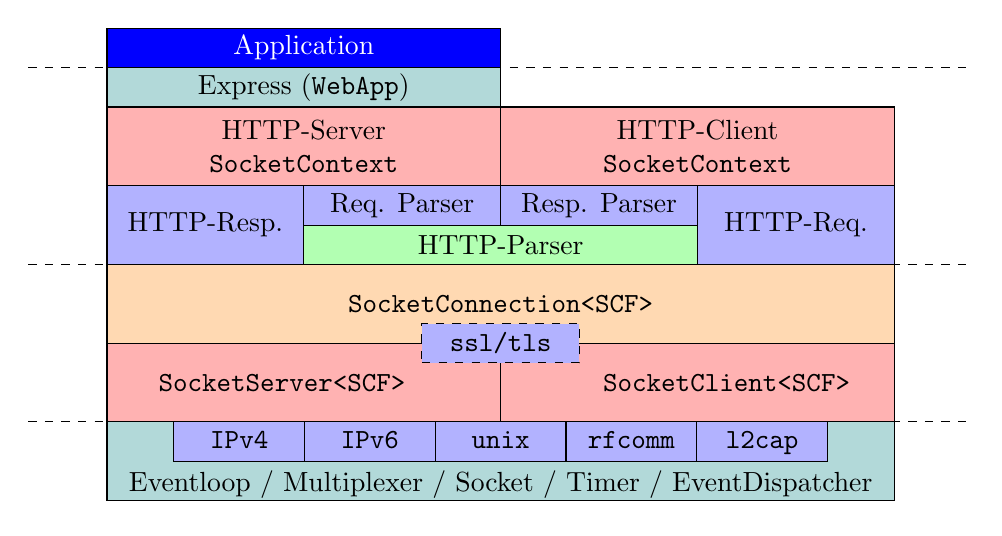
\begin{tikzpicture}
        %%% Start Eventloop / Netzwerk
        \draw node[outer sep=0, draw, fill=teal!30, minimum width=10cm, minimum height=1cm] (em) {};
        \draw (em.center) node [anchor=north] {Eventloop / Multiplexer / Socket / Timer / EventDispatcher};
        \draw (em.north) node[xshift=-0.83cm, outer sep=0, inner sep=0, anchor=north east, draw, fill=blue!30, minimum height=0.5cm, minimum width=1.66cm] (ip6) {\texttt{\strut IPv6}};
        \draw (em.north) node[xshift=+0.83cm,outer sep=0, inner sep=0, anchor=north west, draw, fill=blue!30, minimum height=0.5cm, minimum width=1.66cm] (rfcomm) {\texttt{\strut rfcomm}};
        \draw (em.north) node[outer sep=0, inner sep=0, anchor=north, draw, fill=blue!30, minimum height=0.5cm, minimum width=1.66cm] (unix) {\texttt{\strut unix}};
        \draw (rfcomm.east) node[outer sep=0, inner sep=0, anchor=west, draw, fill=blue!30, minimum height=0.5cm, minimum width=1.66cm] (l2cap) {\texttt{\strut l2cap}};
        \draw (ip6.west) node[outer sep=0, inner sep=0, anchor=east, draw, fill=blue!30, minimum height=0.5cm, minimum width=1.66cm] (ip4) {\texttt{\strut IPv4}};
        %%% End Eventloop / Netzwerk
        %%$ Start draw dashed line above Eventloop-Layer
        \draw (em.north west) + (-1cm, 0) [dashed] -- ++(11cm, 0);
        %%% End draw dashed line above Eventloop-Layer
        %%% Start Lowlevel Server/Client
        \draw (em.north) node[anchor=south east, outer sep=0, draw, fill=red!30, minimum width=5cm, minimum height=1cm] (llst) {\texttt{SocketServer<SCF>\ \ \ \ }};
        \draw (em.north) node[anchor=south west, outer sep=0, draw, fill=red!30, minimum width=5cm, minimum height=1cm] (llct) {\texttt{\ \ \ \ SocketClient<SCF>}};
        %% End Lowlevel Server/Client
        %% Start SocketConnection
        \draw (llst.north east) node[anchor=south, draw, fill=orange!30, inner sep=0, outer sep=0, minimum width=10cm, minimum height=1cm] (sc) {\texttt{SocketConnection<SCF>}};
        %% End SocketConnection

        %% Start SSL/TLS
        \draw (llst.north east) node[outer sep=0, inner sep=0, anchor=center, draw, dashed, fill=blue!30, minimum width=2cm, minimum height=0.5cm] (ssl) {\texttt{ssl/tls}};
        %% End SSL/TLS

        %% Start draw dashed line above SocketConntextion
        \draw (sc.north west) + (-1cm, 0) [dashed] -- ++(11cm, 0);
        %%% End draw dashed line above SocketConnection

        %% Begin HTTP/Express Layer
        \draw (sc.north) node [anchor=south, outer sep=0, inner sep=0, draw, fill=green!30, minimum width=5cm, minimum height=0.5cm] (http-p) {HTTP-Parser};

        \draw (http-p.south west) node[anchor=south east, outer sep=0, inner sep=0, draw, fill=blue!30, minimum width=2.5cm, minimum height=1cm] (http-res) {HTTP-Resp.};

        \draw (http-p.south east) node[anchor=south west, outer sep=0, inner sep=0, draw, fill=blue!30, minimum width=2.5cm, minimum height=1cm] (http-res) {HTTP-Req.};

        \draw (http-p.north west) node[anchor=south west, outer sep=0, inner sep=0, draw, fill=blue!30, minimum width=2.5cm, minimum height=0.5cm] (http-reqp) {Req. Parser};

        \draw (http-p.north east) node[anchor=south east, outer sep=0, inner sep=0, draw, fill=blue!30, minimum width=2.5cm, minimum height=0.5cm] (http-respp) {Resp. Parser};

        \draw (http-respp.north west) node[outer sep=0, inner sep=0, anchor=south west, fill=red!30, draw, minimum width=5cm, minimum height=1cm, align=center] (http-c) {HTTP-Client\\\texttt{SocketContext}};

        \draw (http-reqp.north east) node[outer sep=0, inner sep=0, anchor=south east, fill=red!30, draw, minimum width=5cm, minimum height=1cm, align=center] (http-s) {HTTP-Server\\\texttt{SocketContext}};

        \draw (http-s.north) node[anchor=south, draw, fill=teal!30, outer sep=0, inner sep=0, minimum height=0.5cm, minimum width=5cm] (ex) {Express (\texttt{WebApp})};
        %% End HTTP/Express Layer

        %% Start draw dashed line above SocketConntextion
        \draw (ex.north west) + (-1cm, 0) [dashed] -- ++(11cm, 0);
        %%% End draw dashed line above SocketConnection

        \visible<2>{\draw (ex.north) node[anchor=south, outer sep=0, inner sep=0, draw, fill=blue, minimum width=5cm, minimum height=0.5cm] {\color{white}Application};}

      \end{tikzpicture}
      \caption{Die Eventloop- und Netzwerkschicht im Detail.}
    \end{figure}
  \end{center}
\end{frame}
